% Mini research note for cost audits, numerical coherence, and trust diagnostics.
\documentclass[11pt]{article}
% Shared preamble for the research-note series.
% Create note-specific content in the per-note directory; keep common macros here.
\usepackage[margin=1in]{geometry}
\usepackage[T1]{fontenc}
\usepackage[utf8]{inputenc}
\usepackage{amsmath,amssymb}
\usepackage{booktabs,longtable,array}
\usepackage{graphicx}
\usepackage{float}
\usepackage{enumitem}
\usepackage{xcolor}
\usepackage{hyperref}
\usepackage{caption}
\usepackage{titlesec}
\hypersetup{colorlinks=true, linkcolor=blue!60!black, urlcolor=blue!60!black, citecolor=blue!60!black}
\setlist[itemize]{leftmargin=1.25em, itemsep=0.2em, topsep=0.3em}
\setlist[enumerate]{leftmargin=1.4em, itemsep=0.2em, topsep=0.3em}
\setlength{\parindent}{0pt}
\setlength{\parskip}{0.6em}
\newcommand{\statusbox}[2]{%
  \noindent\fcolorbox{black}{gray!10}{%
    \parbox{\dimexpr\linewidth-2\fboxsep-2\fboxrule\relax}{%
      \textbf{Status:} #1\\#2
    }%
  }
}

% Shared notation helpers for the research-note series.
\newcommand{\Jlin}{J}
\newcommand{\Jphys}{J_{\mathrm{phys}}}
\newcommand{\Jsurf}{J_{\mathrm{surf}}}
\newcommand{\JdB}{J_{\mathrm{dB}}}
\newcommand{\phiopt}{\phi_{\mathrm{opt}}}
\newcommand{\sigmathreedb}{\sigma_{3\mathrm{dB}}}
\newcommand{\Nt}{N_t}
\newcommand{\Nphi}{N_{\phi}}
\newcommand{\Lfiber}{L}
\newcommand{\Pcont}{P}
\newcommand{\band}{\mathcal{B}_{\mathrm{Raman}}}
\newcommand{\todoitem}[1]{\textcolor{red!70!black}{\textbf{TODO:} #1}}


\title{Cost Audit, Numerics Coherence, and Trust Diagnostics}
\author{Fiber Raman Suppression Project}
\date{Evidence snapshot: 2026-04-26}

\begin{document}
\maketitle

\begin{abstract}
This note explains how the project decides whether a Raman-suppression result
is numerically trustworthy. The main lesson is simple: an impressive
suppression number is not enough. The scalar objective, gradient, regularizers,
units, boundary behavior, and diagnostic images must all describe the same
experiment. The cost-audit runs show that changing objective scale or penalty
choice can change both convergence behavior and final depth. The practical
outcome is a trust checklist that every future research note should inherit.
\end{abstract}

\section*{Claim Status}
\statusbox{methodology established; audit matrix incomplete}{The core
numerical rules are stable: report the objective surface, keep gradients on the
same scale as the optimizer cost, inspect boundary and conservation checks, and
include standard images. The older cost-audit matrix is useful but incomplete:
one fiber/power configuration and one sharpness-aware run are still missing.
This note is therefore a trustworthy-methods note, not a claim that every
candidate result has been fully revalidated.}

\section{Question and Thesis}

The research notes in this series compare many different phase masks,
optimizers, basis choices, and fiber settings. Those comparisons only make
sense if they are using the same meaning of ``cost.'' This note asks:
\[
    \text{When should a low Raman cost be trusted as evidence?}
\]

The thesis is that every reported result needs two layers of evidence:
\[
    \text{physics performance} \quad + \quad \text{numerical coherence}.
\]
Physics performance is the Raman-band suppression itself. Numerical coherence
means the objective, gradient, regularization, grid, boundary checks, and plots
all agree about what was optimized.

\subsection*{Intuition Check}

If a graph says a mask reached \(-70\,\mathrm{dB}\), the first question should
not be ``is that good?'' It should be ``what exact scalar function produced
that number, and did the solver really optimize that same scalar function?''
This is the difference between a result and a number that happens to come out
of a script.

\section{The Cost Function}

The physical quantity of interest is the fraction of output spectral energy in
the Raman-shifted band:
\[
    \Jphys(\phi)
    =
    \frac{
        \sum_{\omega_k\in\band} |u_{\omega_k}(L;\phi)|^2\,\Delta\omega
    }{
        \sum_k |u_{\omega_k}(L;\phi)|^2\,\Delta\omega
    }.
\]
The shaped input is
\[
    u_\omega(0;\phi)=u_{\omega,0}\exp(i\phi(\omega)).
\]
The field \(u_\omega(L;\phi)\) comes from the nonlinear fiber propagation
solver. The forward model follows the standard split-step / interaction-picture
fiber-simulation literature \cite{agrawal2019,dudley2006,hult2007}.

The project often reports
\[
    \JdB(\phi)=10\log_{10}\Jphys(\phi).
\]
More negative values mean less Raman-band energy. A change from
\(-30\,\mathrm{dB}\) to \(-60\,\mathrm{dB}\) is not a small cosmetic change:
it is a factor of \(10^3\) in the Raman-band fraction.

\subsection*{Intuition Check}

\(\Jphys\) is a fraction. If \(\Jphys=10^{-5}\), then one part in \(100{,}000\)
of the output spectral energy lies in the Raman band. The dB form is just a
more readable way to display tiny fractions.

\section{Linear Surface Versus Optimizer Surface}

The optimizer does not always see only \(\Jphys\). Some runs include penalties:
\[
    \Jlin(\phi)
    =
    \Jphys(\phi)
    +\lambda_{\mathrm{gdd}}R_{\mathrm{gdd}}(\phi)
    +\lambda_{\mathrm{edge}}R_{\mathrm{edge}}(\phi).
\]
Here \(R_{\mathrm{gdd}}\) discourages extreme curvature in spectral phase, and
\(R_{\mathrm{edge}}\) discourages shaped pulses that put too much time-domain
energy near the FFT-window boundary.

The scalar surface passed to the optimizer is either the linear surface
\[
    \Jsurf(\phi)=\Jlin(\phi),
\]
or the dB surface
\[
    \Jsurf(\phi)=10\log_{10}\Jlin(\phi).
\]
The important rule is that the gradient must match this exact surface:
\[
    \nabla \Jsurf
    =
    \frac{10}{\ln 10}\frac{1}{\Jlin}\nabla \Jlin
    \qquad
    \text{when the dB surface is used.}
\]

The curvature warning is the same idea one derivative later. If
\(F(\phi)=10\log_{10}\Jlin(\phi)\), then the Hessian is not just the linear
Hessian multiplied by a constant:
\[
    \nabla^2 F
    =
    \frac{10}{\ln 10}
    \left(
    \frac{1}{\Jlin}\nabla^2\Jlin
    -
    \frac{1}{\Jlin^2}\nabla\Jlin\nabla\Jlin^{T}
    \right).
\]
So a Hessian-vector product built for the linear physics cost is useful, but it
is not automatically the Hessian of the regularized dB optimizer surface.

\begin{figure}[H]
\centering
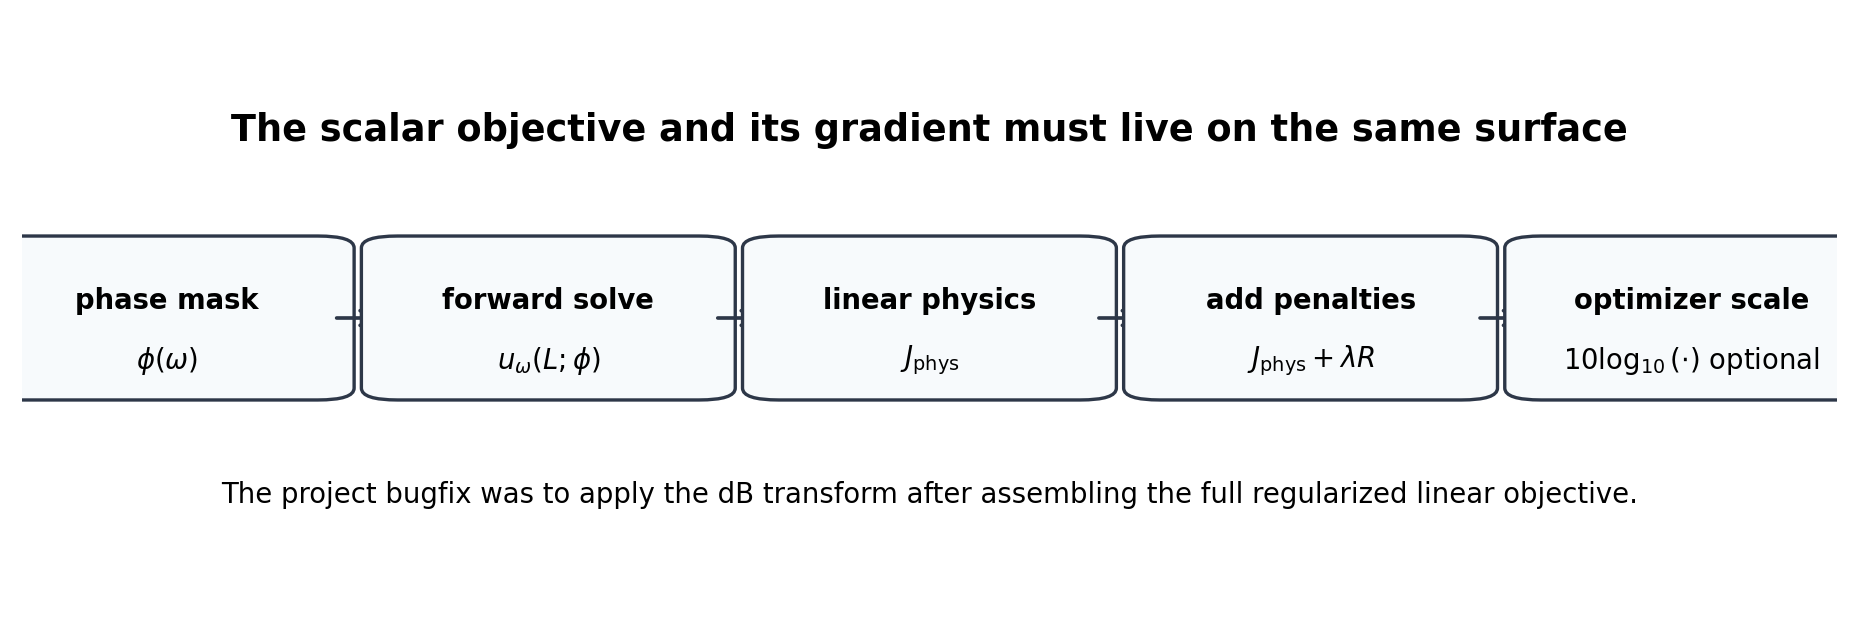
\includegraphics[width=0.94\linewidth]{figures/objective_surface_pipeline.png}
\caption{Objective-surface pipeline. The dB transform belongs after the full
regularized linear objective has been assembled, so the cost and gradient seen
by the optimizer describe the same function.}
\end{figure}

\subsection*{Intuition Check}

The dB transform is like changing from meters to centimeters, except it is
nonlinear. You cannot change the units of the cost and forget to change the
gradient. If the cost is in dB but the gradient is still linear, the optimizer
is following directions for the wrong map.

\subsection*{What The Regularizers Mean}

The curvature penalty is a discrete second-difference penalty on spectral
phase:
\[
    R_{\mathrm{gdd}}(\phi)
    =
    \sum_{i=2}^{\Nt-1}
    \frac{\left(\phi_{i+1}-2\phi_i+\phi_{i-1}\right)^2}{\Delta\omega^3},
    \qquad
    \Delta\omega=\frac{2\pi}{\Nt\Delta t}.
\]
This is not trying to prove the phase is physically optimal. It is a numerical
pressure against very sharp pixel-to-pixel curvature.

The boundary penalty measures how much shaped input energy sits near the
beginning and end of the time window:
\[
    R_{\mathrm{edge}}(\phi)
    =
    \frac{\sum_{t_j\in\mathrm{edge}}|u(t_j,0;\phi)|^2}
         {\sum_j |u(t_j,0;\phi)|^2}.
\]
The trust report separately checks both input and output edge fractions. This
matters because a result can look deep if the pulse is being pushed into the
numerical window boundary.

\subsection*{Intuition Check}

The curvature penalty says ``do not use a wildly jagged phase unless it really
helps.'' The edge penalty says ``do not win by hiding energy near the edge of
the simulation box.''

\section{Gauge Fixing: What Phase Structure Counts?}

Not every part of \(\phi(\omega)\) is physically meaningful for the comparison
we want to make. A constant phase does not change intensity. A linear spectral
phase mainly shifts the pulse in time. Those two directions are treated as
gauge-like directions:
\[
    \mathcal{G}=\operatorname{span}\{1,\omega-\bar{\omega}\}.
\]
For shape comparisons, the project projects them out:
\[
    \phi_{\perp}=(I-P_{\mathcal{G}})\phi.
\]

\begin{figure}[H]
\centering
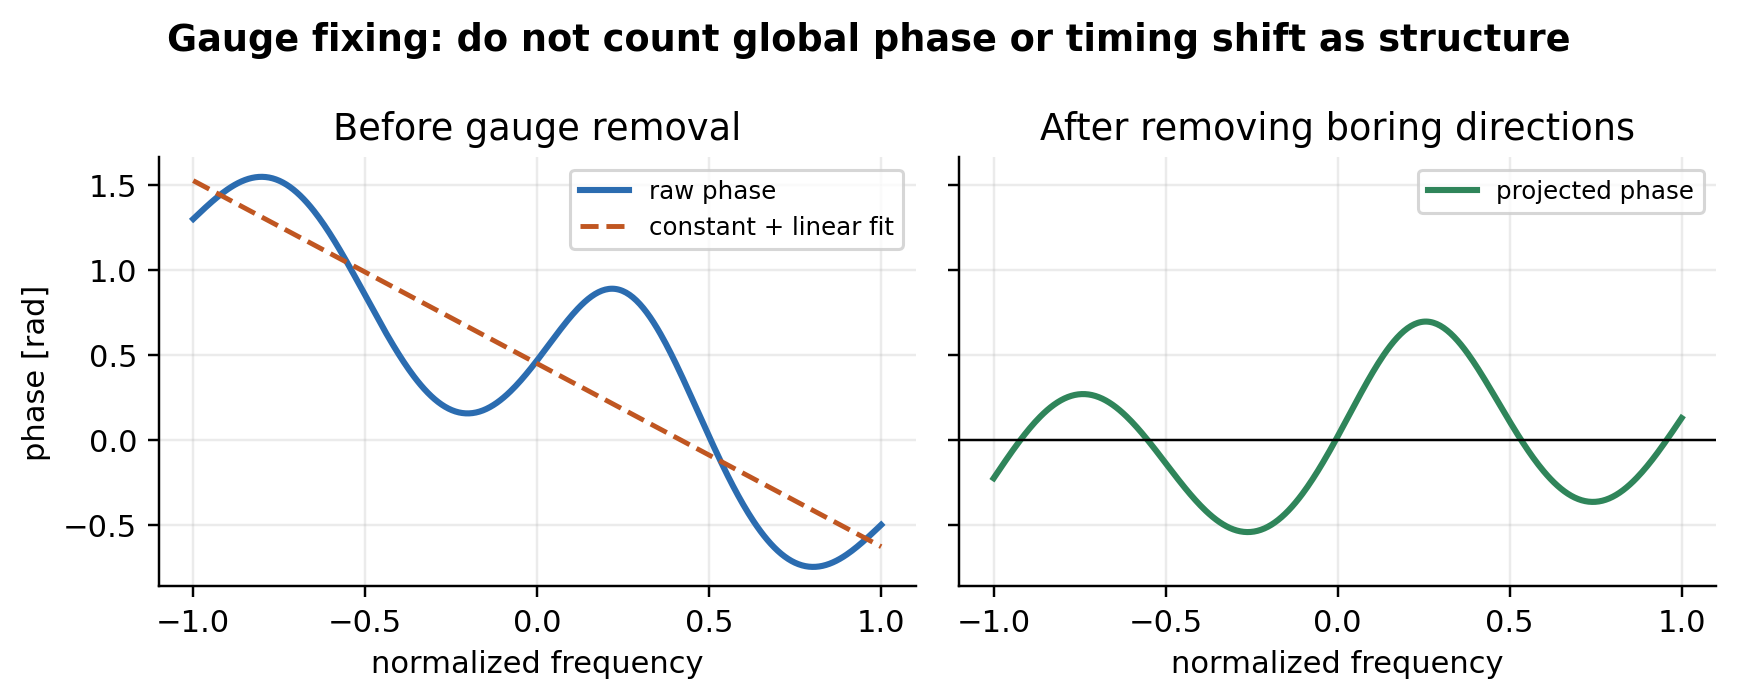
\includegraphics[width=0.86\linewidth]{figures/gauge_projection_clean.png}
\caption{Gauge fixing removes the constant and linear pieces of spectral
phase. The remaining curve is the part that should be compared when asking
whether two masks have the same meaningful shape.}
\end{figure}

\subsection*{Intuition Check}

Quick version: ``subtract off the boring directions before comparing masks.''
Global phase and timing shift can make two curves look different even when
they represent the same useful pulse-shaping idea.

\section{Implementation Surface}

\begin{center}
\footnotesize
\begin{tabular}{>{\raggedright\arraybackslash}p{0.29\linewidth}
                >{\raggedright\arraybackslash}p{0.61\linewidth}}
\toprule
\textbf{Component} & \textbf{Numerical responsibility} \\
\midrule
Raman optimization library &
Builds the single-mode Raman cost and adjoint gradient, including optional
regularizers and the dB objective transform. \\
Objective-surface helper &
Records the scalar objective surface in machine-readable form so trust reports
state whether the run used a linear or dB scale. \\
Numerical trust reporter &
Builds pass/marginal/suspect reports for determinism, boundary energy,
conservation, gradient checks, and cost-surface metadata. \\
Standard-image helper &
Writes the required phase diagnostic, optimized evolution, and unshaped
control evolution images after an optimization run. \\
Cost-audit workflow &
Runs the comparison matrix over objective variants and fiber/power settings. \\
\bottomrule
\end{tabular}
\end{center}

The key code invariant is that regularizers are added on the linear surface
first. If a dB objective is requested, the dB transform is then applied to the
combined scalar objective and to the combined gradient.

\section{Cost-Audit Evidence}

The cost-audit matrix compared objective variants across two completed
fiber/power configurations. Setup A is a short, low-power SMF-28 case
\((L=0.5\,\mathrm{m}, P=0.05\,\mathrm{W})\). Setup B is a longer, higher-power
SMF-28 case \((L=5.0\,\mathrm{m}, P=0.2\,\mathrm{W})\). The missing setup is an
HNLF case that should not be summarized as completed yet.

The variants were: direct linear cost, dB-scaled cost, curvature-regularized
cost, and a sharpness-aware cost. The point is not that one variant wins every
time. The point is that changing the scalar surface changes the optimization
path enough that notes must name the surface explicitly.

\begin{figure}[H]
\centering
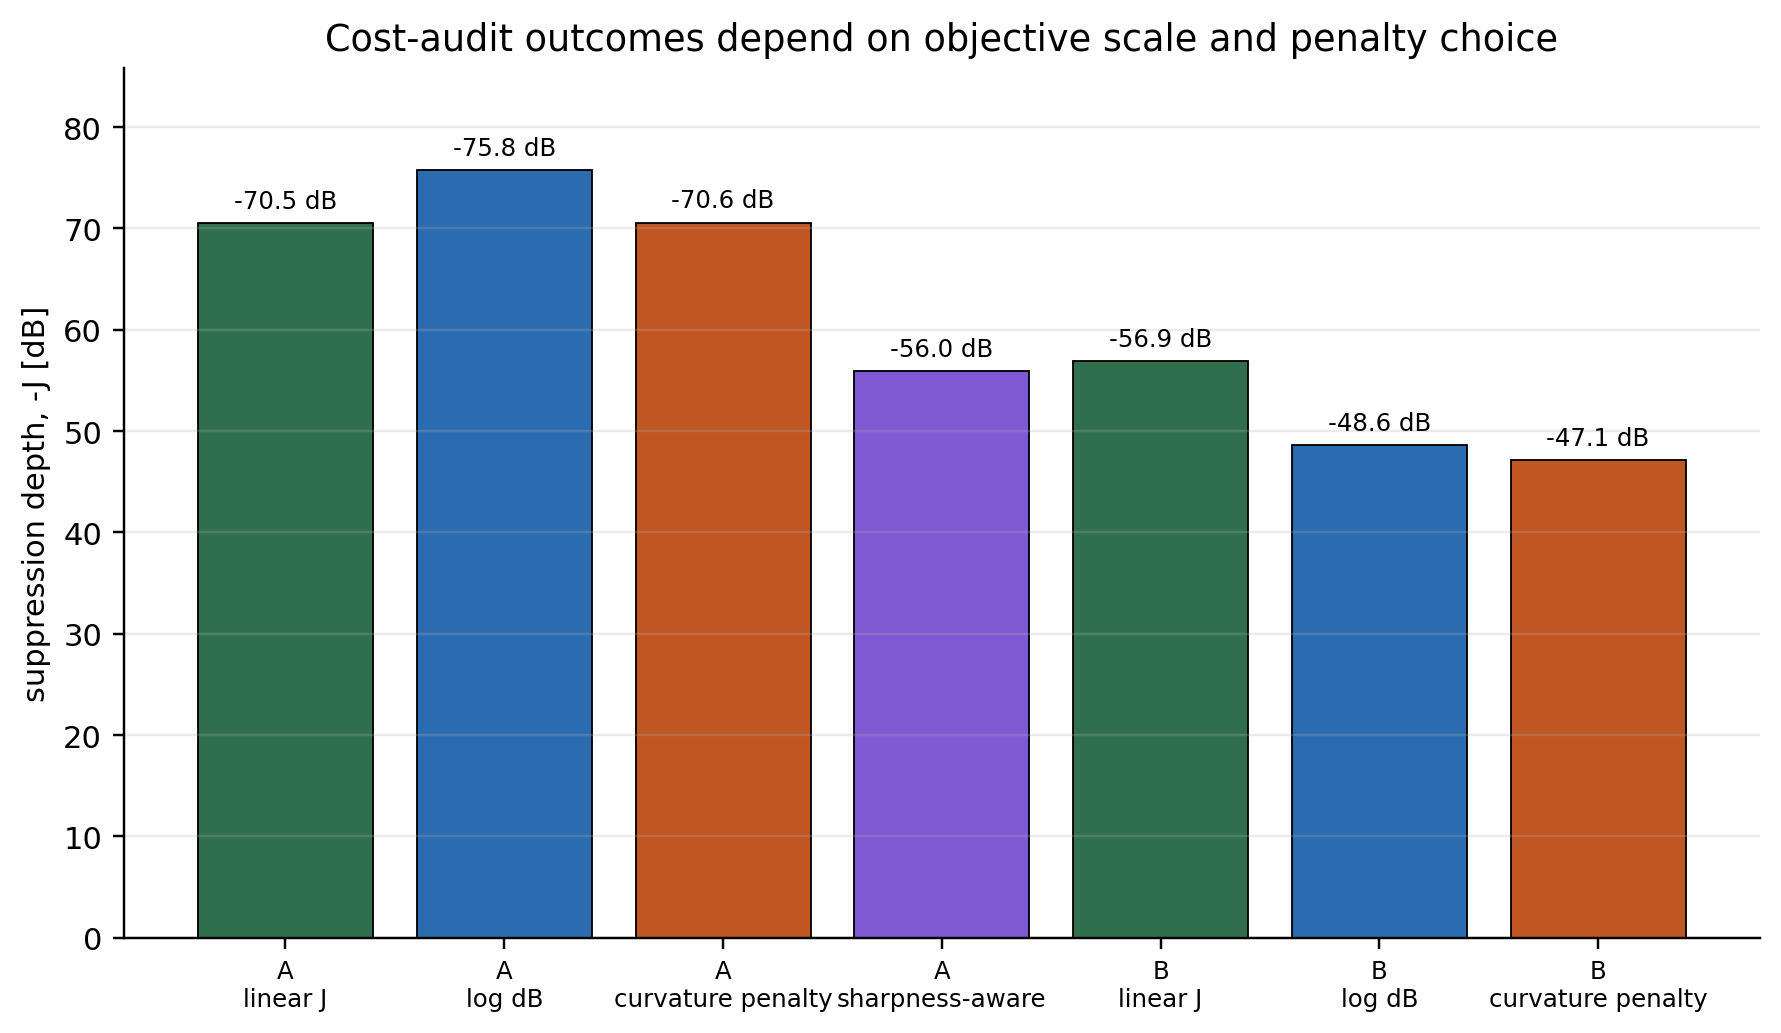
\includegraphics[width=0.92\linewidth]{figures/cost_audit_depth_summary.png}
\caption{Completed cost-audit outcomes. The final suppression depth depends on
the objective scale and penalty choice, so results should always state which
surface was optimized.}
\end{figure}

\begin{figure}[H]
\centering
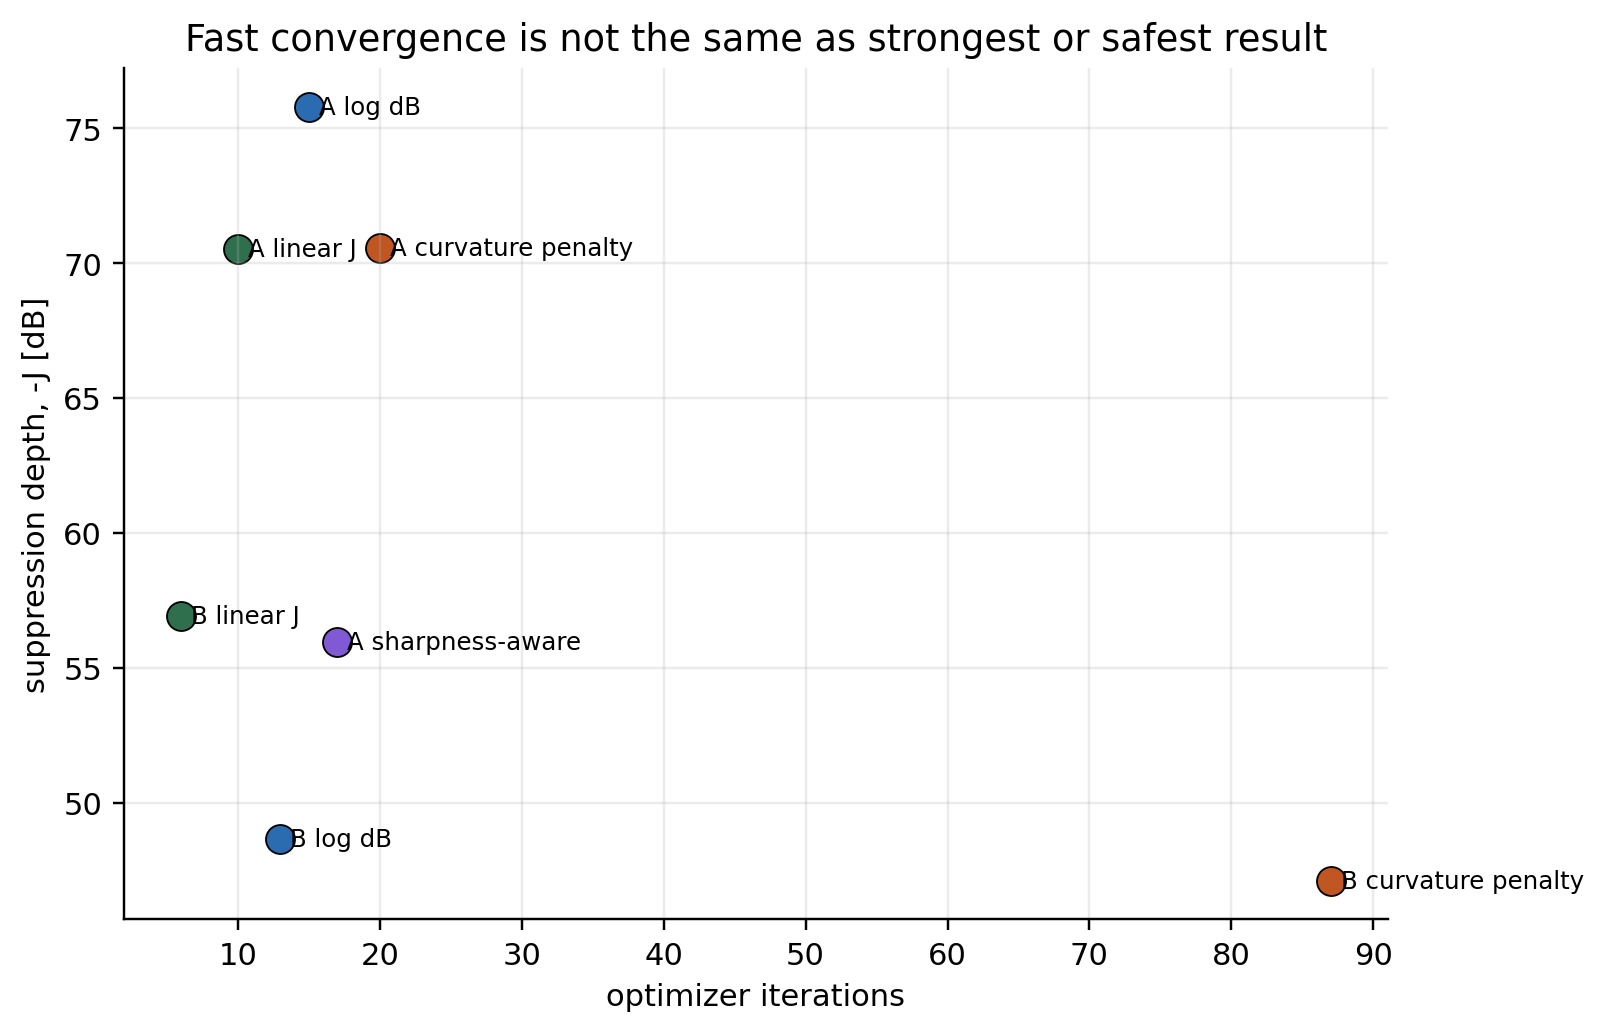
\includegraphics[width=0.82\linewidth]{figures/cost_audit_iteration_tradeoff.png}
\caption{Iteration-depth tradeoff. Fast convergence, deepest native depth, and
best numerical trust are related but not identical goals.}
\end{figure}

\begin{center}
\scriptsize
\setlength{\tabcolsep}{3pt}
\begin{tabular}{@{}>{\raggedright\arraybackslash}p{0.09\linewidth}
                >{\raggedright\arraybackslash}p{0.17\linewidth}
                >{\raggedright\arraybackslash}p{0.14\linewidth}
                >{\raggedright\arraybackslash}p{0.10\linewidth}
                >{\raggedright\arraybackslash}p{0.34\linewidth}@{}}
\toprule
\textbf{Setup} & \textbf{variant} & \textbf{final \(J\)} &
\textbf{iterations} & \textbf{reading} \\
\midrule
A & linear \(J\) & \(-70.53\,\mathrm{dB}\) & 10 &
strong and fast, but linear scale can become tiny and ill-conditioned. \\
A & dB surface & \(-75.79\,\mathrm{dB}\) & 15 &
deepest completed result in this audit set. \\
A & curvature penalty & \(-70.57\,\mathrm{dB}\) & 20 &
similar depth with explicit smoothness pressure. \\
A & sharpness-aware & \(-55.96\,\mathrm{dB}\) & 17 &
shallower because the objective asks for local stability, not only depth. \\
B & linear \(J\) & \(-56.93\,\mathrm{dB}\) & 6 &
deepest completed result for this setup. \\
B & dB surface & \(-48.64\,\mathrm{dB}\) & 13 &
less deep here; objective scale is not automatically better in every regime. \\
B & curvature penalty & \(-47.10\,\mathrm{dB}\) & 87 &
slowest completed run in this audit set. \\
\bottomrule
\end{tabular}
\end{center}

\subsection*{Intuition Check}

The audit does not say ``always use the dB objective.'' It says ``say what you
used, and do not compare runs as if the objective surface were irrelevant.''
Changing the surface can change the path, the convergence criterion, and the
final mask.

\section{Trust Diagnostics}

The numerical trust report turns scattered checks into a repeatable gate:

\begin{figure}[H]
\centering
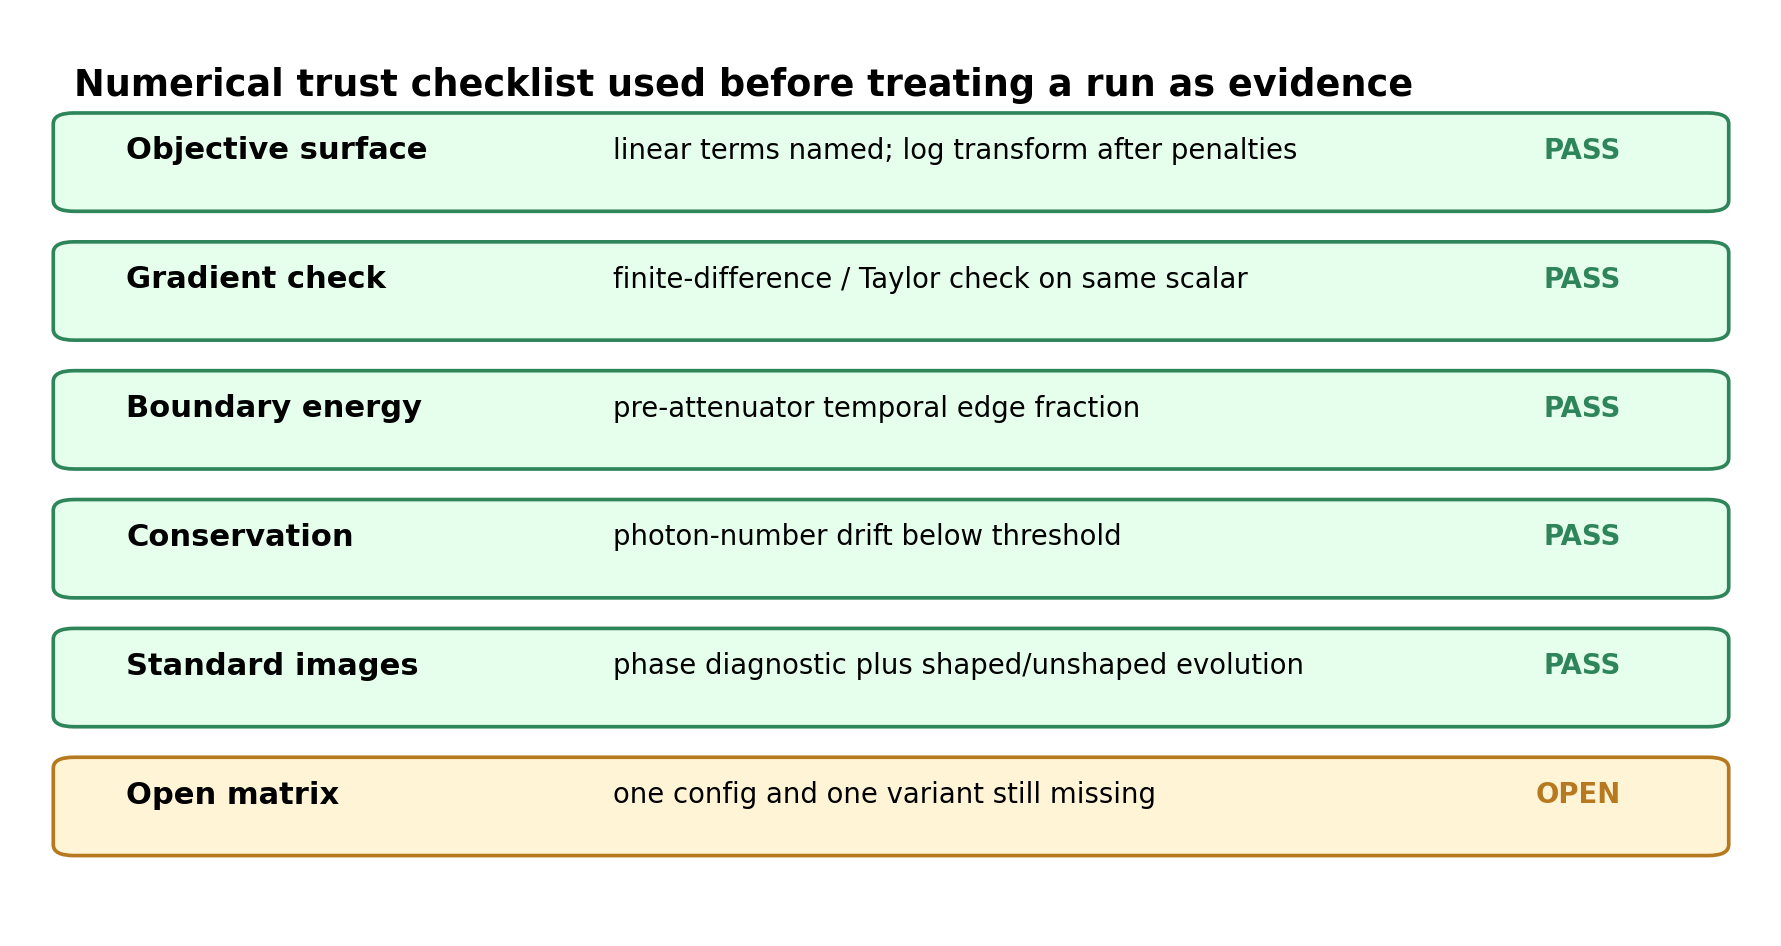
\includegraphics[width=0.90\linewidth]{figures/trust_gate_checklist.png}
\caption{Trust checklist. A result can be visually exciting and still be
marked open or suspect if the objective, boundary, conservation, gradient, or
standard-image evidence is incomplete.}
\end{figure}

The most important checks are:
\begin{itemize}
    \item \textbf{Objective surface:} the report must say whether the scalar
    surface was linear or dB-scaled, and which penalties were included.
    \item \textbf{Gradient validation:} finite-difference or Taylor checks must
    compare against the same scalar objective that the optimizer sees.
    \item \textbf{Boundary energy:} time-domain energy near the FFT-window edge
    is checked before the absorber can hide it.
    \item \textbf{Conservation:} photon-number drift should stay below the
    configured pass or marginal thresholds.
    \item \textbf{Standard images:} the PDF should show the phase diagnostic
    and corresponding spectral evolution, plus an unshaped control.
\end{itemize}

\begin{center}
\small
\resizebox{\linewidth}{!}{%
\begin{tabular}{>{\raggedright\arraybackslash}p{0.34\linewidth}
                >{\raggedleft\arraybackslash}p{0.18\linewidth}
                >{\raggedleft\arraybackslash}p{0.20\linewidth}
                >{\raggedright\arraybackslash}p{0.22\linewidth}}
\toprule
\textbf{Metric} & \textbf{Pass} & \textbf{Marginal} & \textbf{Why it matters} \\
\midrule
Max edge fraction & \(\le 10^{-3}\) & \(\le 10^{-2}\) &
Checks whether the pulse fits in the time window. \\
Photon-number drift & \(\le 10^{-4}\) & \(\le 10^{-3}\) &
Checks whether propagation is numerically coherent. \\
Gradient max relative error & \(\le 5\times10^{-2}\) &
\(\le 10^{-1}\) & Checks whether the optimizer direction matches the scalar
cost. \\
\bottomrule
\end{tabular}}
\end{center}

\subsection*{Intuition Check}

Think of the trust report as a lab notebook checklist. It does not prove the
physics is publishable by itself, but it catches common ways a simulation can
look better than it deserves.

\section{Representative Standard Images}

The standard images are not decoration. They are part of the audit. The phase
diagnostic tells us whether the mask is smooth, wrapped, pixel-like, or
dominated by gauge directions. The heat map shows whether the shaped pulse
actually changes the spectral evolution relative to the control.

\begin{figure}[p]
\centering

\includegraphics[height=0.47\textheight]{figures/control_no_optimization_phase_diagnostic.png}
\vspace{0.5em}


\includegraphics[height=0.31\textheight]{figures/control_no_optimization_evolution.png}
\caption{No-optimization control. A flat phase and the corresponding unshaped
evolution give the visual reference for deciding whether a shaped result is
actually suppressing Raman-band growth.}
\end{figure}

\begin{figure}[p]
\centering
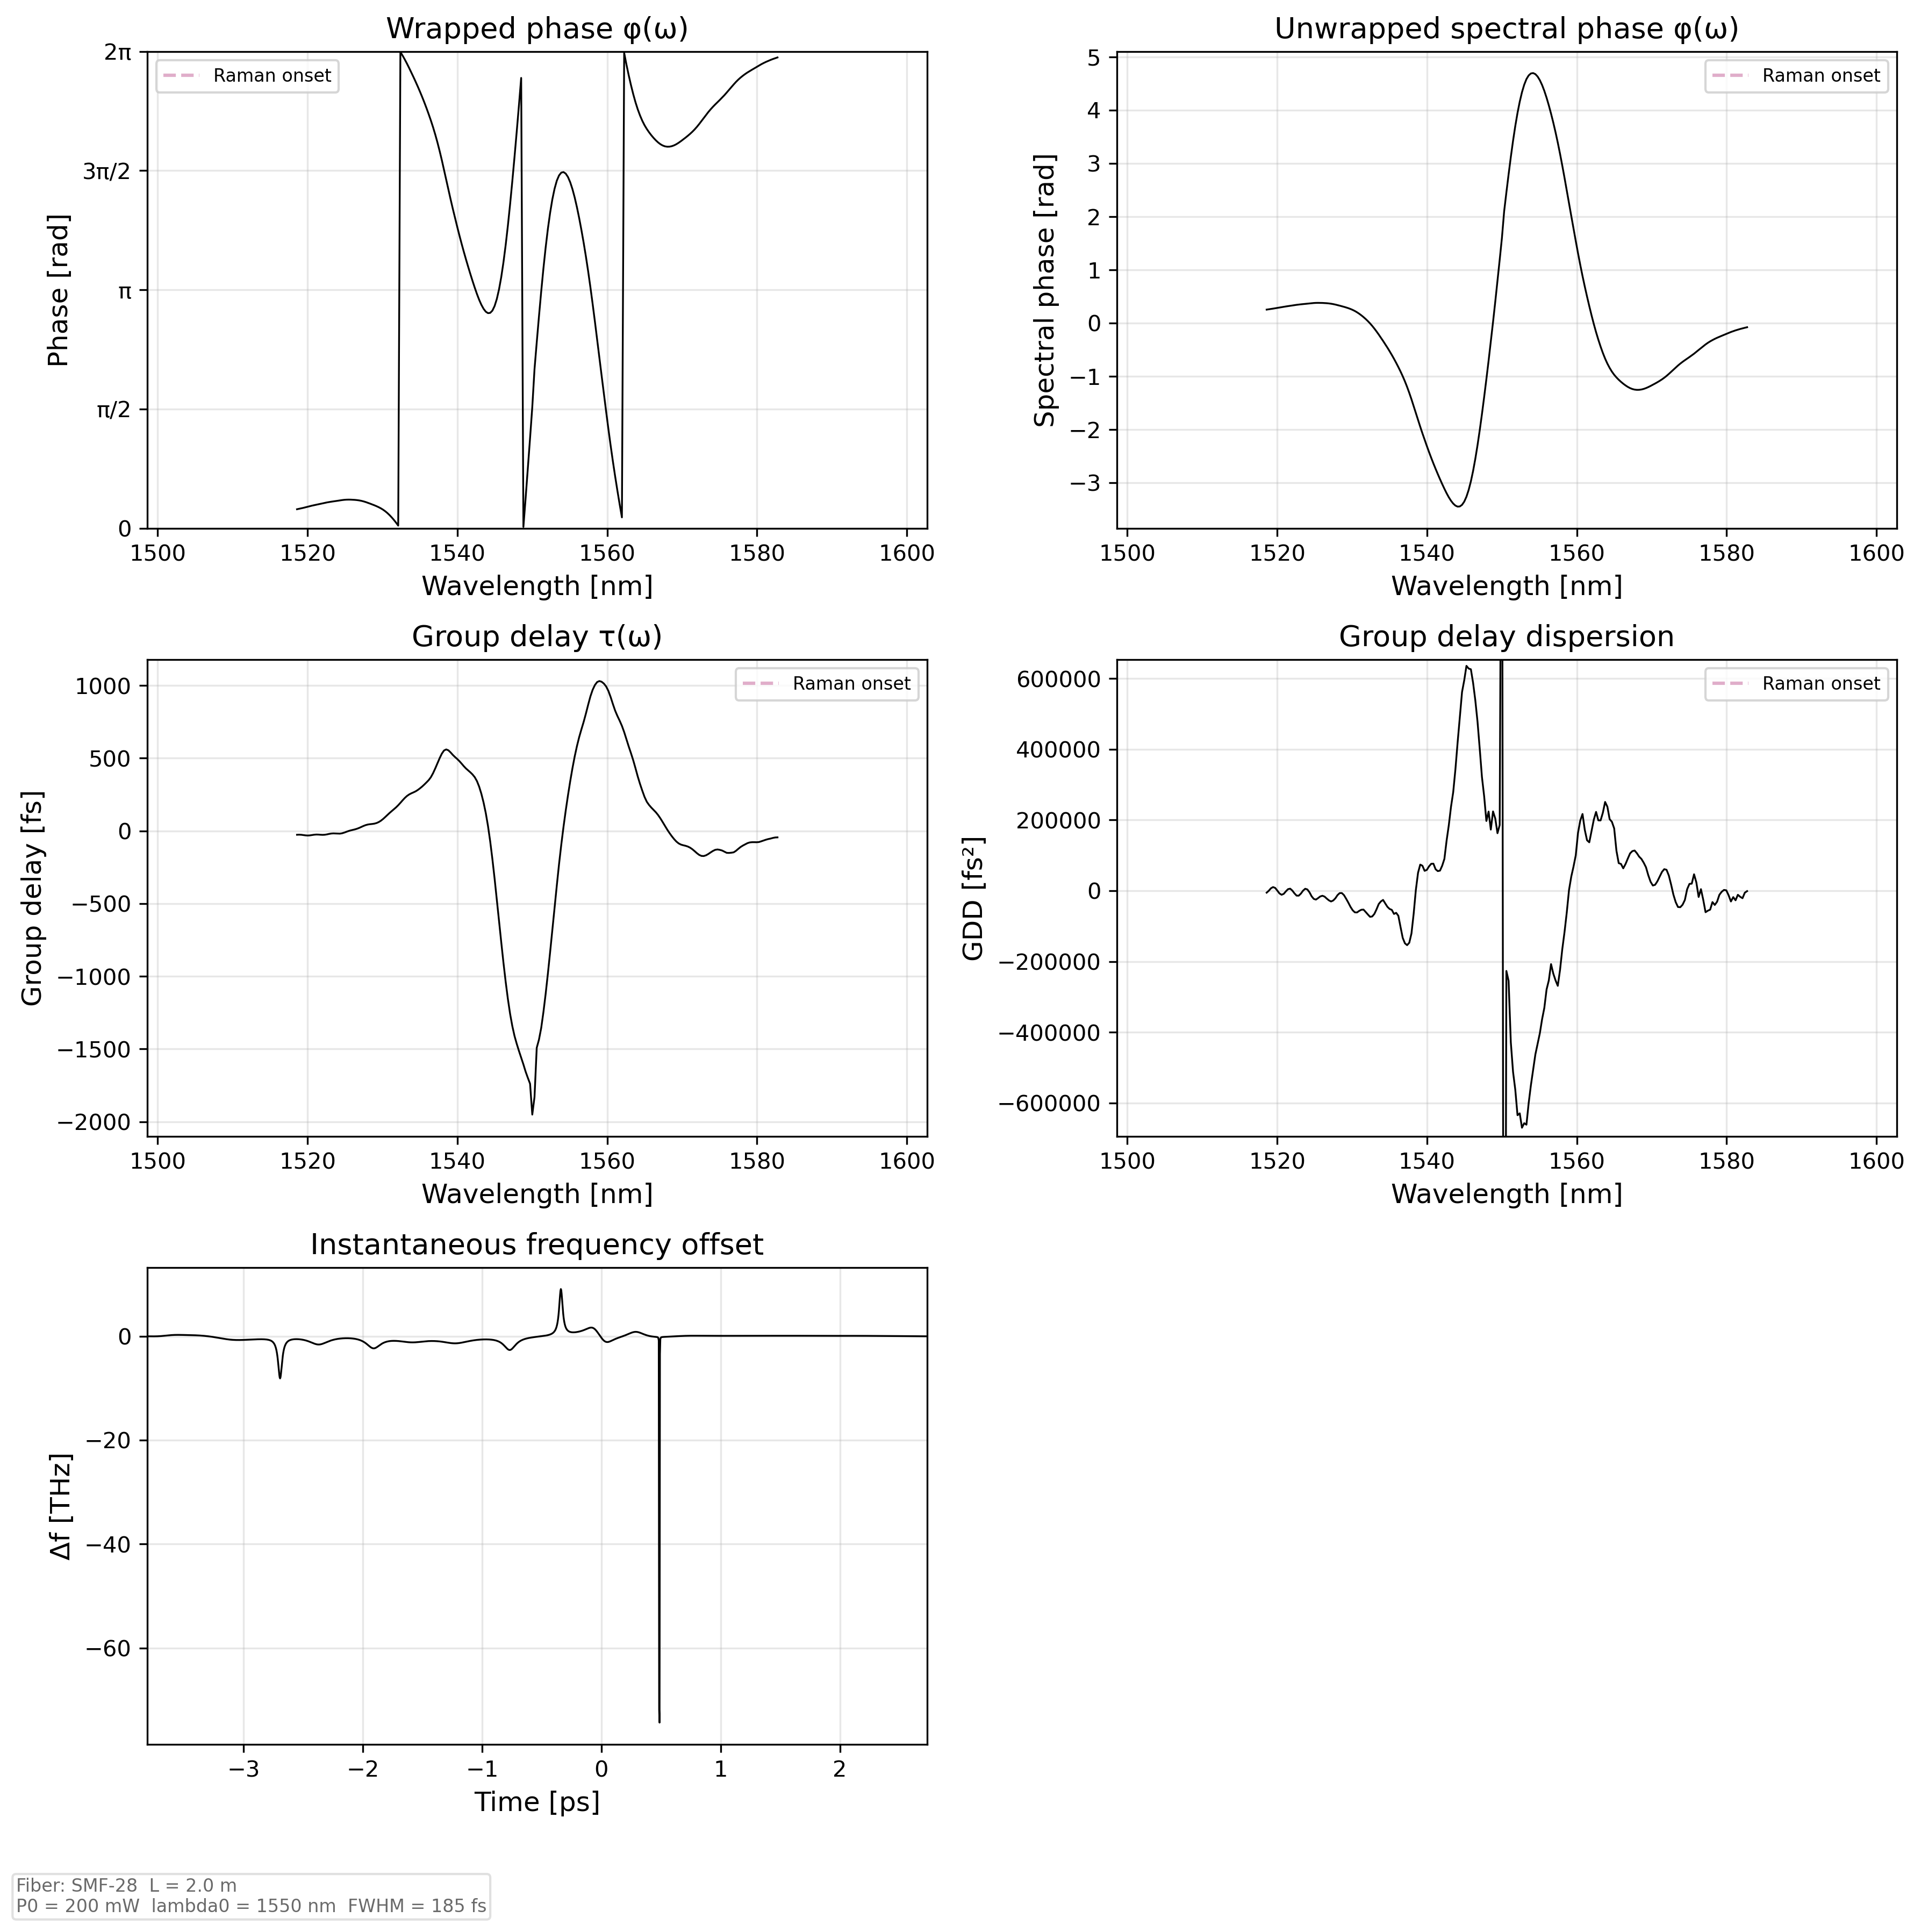
\includegraphics[height=0.47\textheight]{figures/canonical_result_phase_diagnostic.png}
\vspace{0.5em}

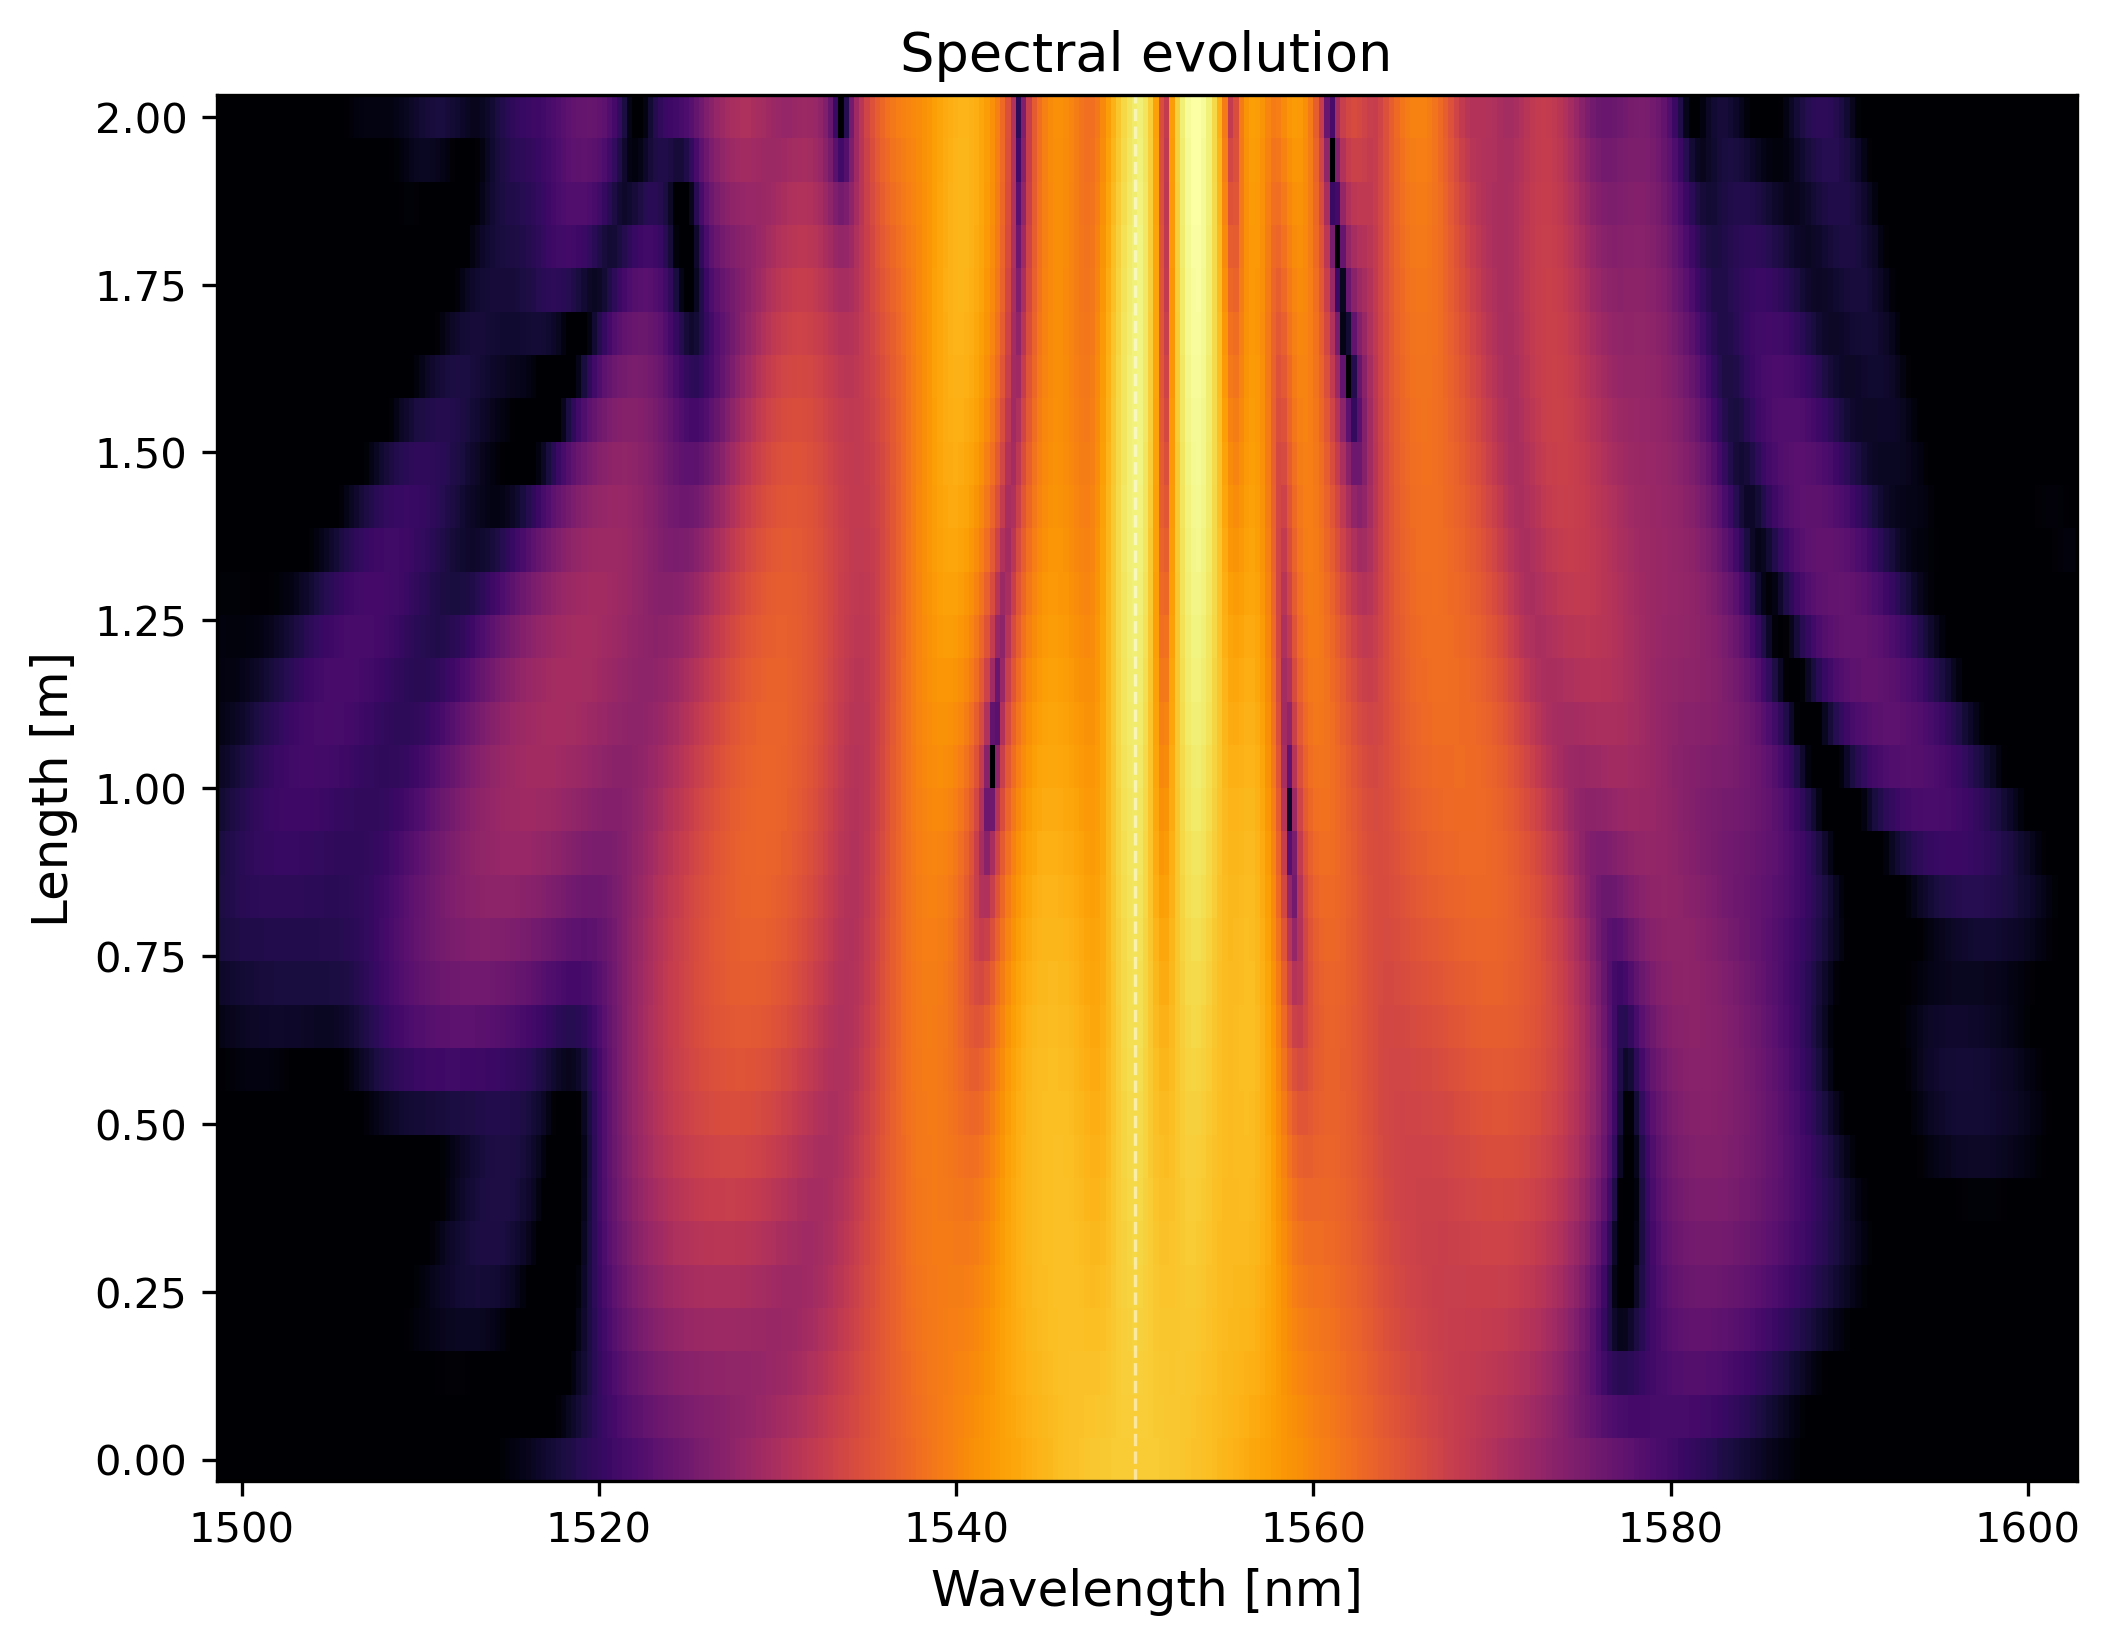
\includegraphics[height=0.31\textheight]{figures/canonical_result_evolution.png}
\caption{Representative shaped result. The phase diagnostic and heat map must
be read together: the curve shows what mask was applied, and the heat map shows
how the spectrum evolved under that mask.}
\end{figure}

\clearpage
\section{Current Limits and Missing Evidence}

The cost-audit lane is strong enough to define project standards, but it is
not complete enough to settle every optimizer comparison.

\begin{itemize}
    \item One planned fiber/power configuration in the audit matrix is still
    missing all objective variants.
    \item One sharpness-aware run is missing from the completed second setup.
    \item Hessian and trust-region tools must always state which scalar surface
    their Hessian-vector products represent. A linear-cost Hessian is useful,
    but it is not automatically the Hessian of a regularized dB objective.
    \item Very deep results, roughly the \(-60\) to \(-80\,\mathrm{dB}\) range,
    should be treated carefully because tiny linear fractions can expose
    solver tolerance, scaling, and conditioning issues.
    \item Mixed unit conventions remain a readability and conditioning hazard.
    The code works with them, but outward notes should be explicit about ps,
    THz, rad/ps, seconds, and normalized frequency whenever a formula depends
    on units.
\end{itemize}

\subsection*{Intuition Check}

The right scientific posture is not pessimism. It is bookkeeping. A result is
much easier to defend when the note already says what was checked, what was
not checked, and what would change the conclusion.

\section{Presentation Capsule}

If this note becomes a methods-quality slide, the clean message is:
\begin{itemize}
    \item The scalar objective, gradient, regularizers, and dB transform must all describe the same optimization surface.
    \item Gauge directions matter because constant and timing-like phase changes can look like structure without changing the physical claim.
    \item Standard images are a verification tool: every important phase profile should be paired with the heat map that shows what happened in propagation.
    \item This note is the credibility layer for the project; it is not the place to sell the most dramatic Raman before/after result.
\end{itemize}

\section{Reproduction Capsule}

For a future rerun, use the cost-audit driver on the heavy machine rather than
running substantial simulations on the editing host:
\[
\texttt{julia -t auto --project=. scripts/research/cost\_audit/cost\_audit\_driver.jl}.
\]
The expected durable outputs are result payloads, a summarized audit table,
trust metadata, and standard images for any run that produces an optimized
phase. For documentation production, the minimum acceptable evidence package
for a candidate is:
\begin{enumerate}
    \item objective-surface statement: linear or dB, with penalties listed;
    \item final Raman fraction in dB and, when needed, the underlying linear
    fraction;
    \item gradient or Taylor validation status;
    \item boundary and conservation verdicts;
    \item no-optimization control image;
    \item phase diagnostic plus corresponding spectral-evolution heat map.
\end{enumerate}

\section{Sources and References}

\begin{thebibliography}{9}

\bibitem{agrawal2019}
G. P. Agrawal.
\textit{Nonlinear Fiber Optics}, 6th ed.
Academic Press, 2019.
\url{https://www.sciencedirect.com/book/9780128170427/nonlinear-fiber-optics}

\bibitem{dudley2006}
J. M. Dudley, G. Genty, and S. Coen.
``Supercontinuum generation in photonic crystal fiber.''
\textit{Reviews of Modern Physics}, 78, 1135--1184, 2006.
\url{https://doi.org/10.1103/RevModPhys.78.1135}

\bibitem{hult2007}
J. Hult.
``A fourth-order Runge-Kutta in the interaction picture method for simulating
supercontinuum generation in optical fibers.''
\textit{Journal of Lightwave Technology}, 25(12), 3770--3775, 2007.
\url{https://doi.org/10.1109/JLT.2007.909373}

\bibitem{nocedal2006}
J. Nocedal and S. J. Wright.
\textit{Numerical Optimization}, 2nd ed.
Springer, 2006.
\url{https://doi.org/10.1007/978-0-387-40065-5}

\bibitem{higham2002}
N. J. Higham.
\textit{Accuracy and Stability of Numerical Algorithms}, 2nd ed.
SIAM, 2002.
\url{https://doi.org/10.1137/1.9780898718027}

\bibitem{frigo2005}
M. Frigo and S. G. Johnson.
``The Design and Implementation of FFTW3.''
\textit{Proceedings of the IEEE}, 93(2), 216--231, 2005.
\url{https://doi.org/10.1109/JPROC.2004.840301}

\end{thebibliography}

\end{document}
